\section{Impact of Clock Stability on Duty Cycling, Bandwidth, and Power Consumption}
\label{sec:power}

It is generally assumed that using a more stable clock will improve the duty
cycling capabilities of an embedded system and save bandwidth since less 
frequent resynchronizations are necessary. Dutta
showed in \cite{dutta2007procrastination} that the lower bound of a clock with
a stability of $\pm 50$ppm is a duty cycle of 0.01\% for a scheduled
communication MAC protocol. But, how much additional power and bandwidth could be saved by
employing a more stable clock, considering that a more stable clock consumes
more power? 

\subsection{Clock Stability and Duty Cycling}
Let us compare two systems, $A$ and $B$. Both systems have the same sleep power
consumption $P_s$ and active power consumption $P_a$.  Each node has a local
clock source with stability $s_A$ and $s_B$ (in $Hz/Hz$) that consume power $P_{cA}$ and $P_{cB}$,
respectively. Additionally, we assume that both platforms have the same duty
cycle ratio $DC$ between sleep ($T_s$) and active time ($T_a$). However, in order
to communicate with their peers, both systems include a guard time that is
proportional to their local clock source's stability $T_{gX} = 2 \cdot T_s \cdot
s_X$, where $s_X$ is the system's local clock stability. This guard time
allows the nodes to compensate for the drift in their clock while asleep by starting the synchronization
process early enough to ensure that both nodes are awake when the active period starts.

Given these definitions, we can calculate the average power consumption of the
system and its clock in the sleep, active and guard periods as follows:
\begin{equation}
	P_X = \frac{T_s \cdot (P_s + P_{cX}) + (T_{gX} + T_a) \cdot (P_a + P_{cX})}{T_s + T_s + T_{gX}}.
\end{equation}

Where $X$ is either $A$ or $B$. Let us also assume that $s_A > s_B$ and $P_{cA} < P_{cB}$. In order for
system $B$ to be more efficient than system $A$ we have to show that
\begin{equation}
	P_A > P_B,
\end{equation}
and thus
\begin{eqnarray}
	\lefteqn{\frac{T_s \cdot (P_s + P_{cA}) + (T_{gA} + T_a) \cdot (P_a + P_{cA})}{T_s + T_a + T_{gA}}  > } \nonumber \\
	& & \frac{T_s \cdot (P_s + P_{cB}) + (T_{gB} + T_a) \cdot (P_a +
	P_{cB})}{T_s + T_a + T_{gB}}.\label{eq:1}
\end{eqnarray}

We now assume that the clock of system $A$ is an inexpensive low frequency crystal as
found in many embedded systems. These crystals consume very little power, and thus
$P_{cA} \sim 0$. Using this assumption, Equation \ref{eq:1} can be simplified to
\begin{equation}
%	P_{cB} & < & \frac{T_s P_s + (T_{gA} + T_a) \cdot P_a}{T_s + T_a + T_{gA}}
%	\nonumber \\
%	& & - \frac{T_s P_s + (T_{gB} + T_a) \cdot P_a}{T_s + T_a + T_{gB}} \nonumber \\
P_{cB} < \frac{2\cdot T_s^2\cdot(P_a-P_s)\cdot(s_1-s_2)}{(T_s\cdot(1+2s_1)+T_a)(T_s\cdot(1+2s_2)+T_a)},
	\label{eq:2}
\end{equation}
where we replaced $T_{gA}$ and $T_{gB}$ with its respective definition. We can
now observe that $DC=T_a/(T_a + T_s)$ is the duty cycle of the system, and if
we assume that $s_1, s_2 << 1$, we get
\begin{equation}
	P_{cB} < 2 \cdot [1-DC]^2\cdot (P_a-P_s) \cdot (s_1-s_2).
\end{equation}
Further assuming that $DC << 1$, $P_s \rightarrow 0$, and $s_1 >> s_2$ we find that
\begin{equation}
	P_{cB} < 2 \cdot P_a \cdot s_1.
\end{equation}

This shows that in order for system $B$ to be more power efficient than system
$A$, the clock system used in system $B$ has to use less power than the active
power consumption multiplied by twice the precision of system $A$'s clock
stability. For example, if we assume that $P_a=1W$, $s_1=50 ppm$, and $s_2=1
ppm$ (in order to satisfy $s_1 >> s_2$) then $P_{cB} < 100 \mu W$. We
currently don't know of a technology that can achieve a clock stability of
$1ppm$ with a power budget of less than $100 \mu W$. The closest we could find
on the current market is the MAXIM DS32BC35 \cite{maxim2008ds32b35} which is
an RTC with integrated 32kHz TCXO, and consumes about 600mW for a stability of
$\pm 3.5ppm$. However, we also ignored the fact that time synchronization
protocols, such as FTSP \cite{maroti2004ftsp}, can estimate the current clock
drift very accurately and thus, as long as the temperature doesn't change too
quickly, can improve the duty cycling of an embedded system without using a
higher stability clock source.


\subsection{Bandwidth Benefits}

It is trivial to see that a time synchronization protocol based on a less
temperature stable clock needs to resynchronize more often, than one based on
a more stable clock. But how much is the difference? In the simplest case,
which represents an upper bound, the time synchronization algorithm assumes
the worst case drift $s_{\max}$ and calculates the necessary resynchronization
time interval $T_r$ based on a maximum allowed time synchronization error
$\epsilon$

\begin{equation}
    T_r < \frac{\epsilon}{s_{\max}}.
\end{equation}

This is a very conservative estimate and doesn't include the fact that a time
synchronization protocol can calculate the current clock drift. Additionally,
if we have knowledge of how fast temperature changes in the environment where
the system is located, then a much better estimate of $T_r$ can be found. 

\begin{figure}
    \begin{center}
        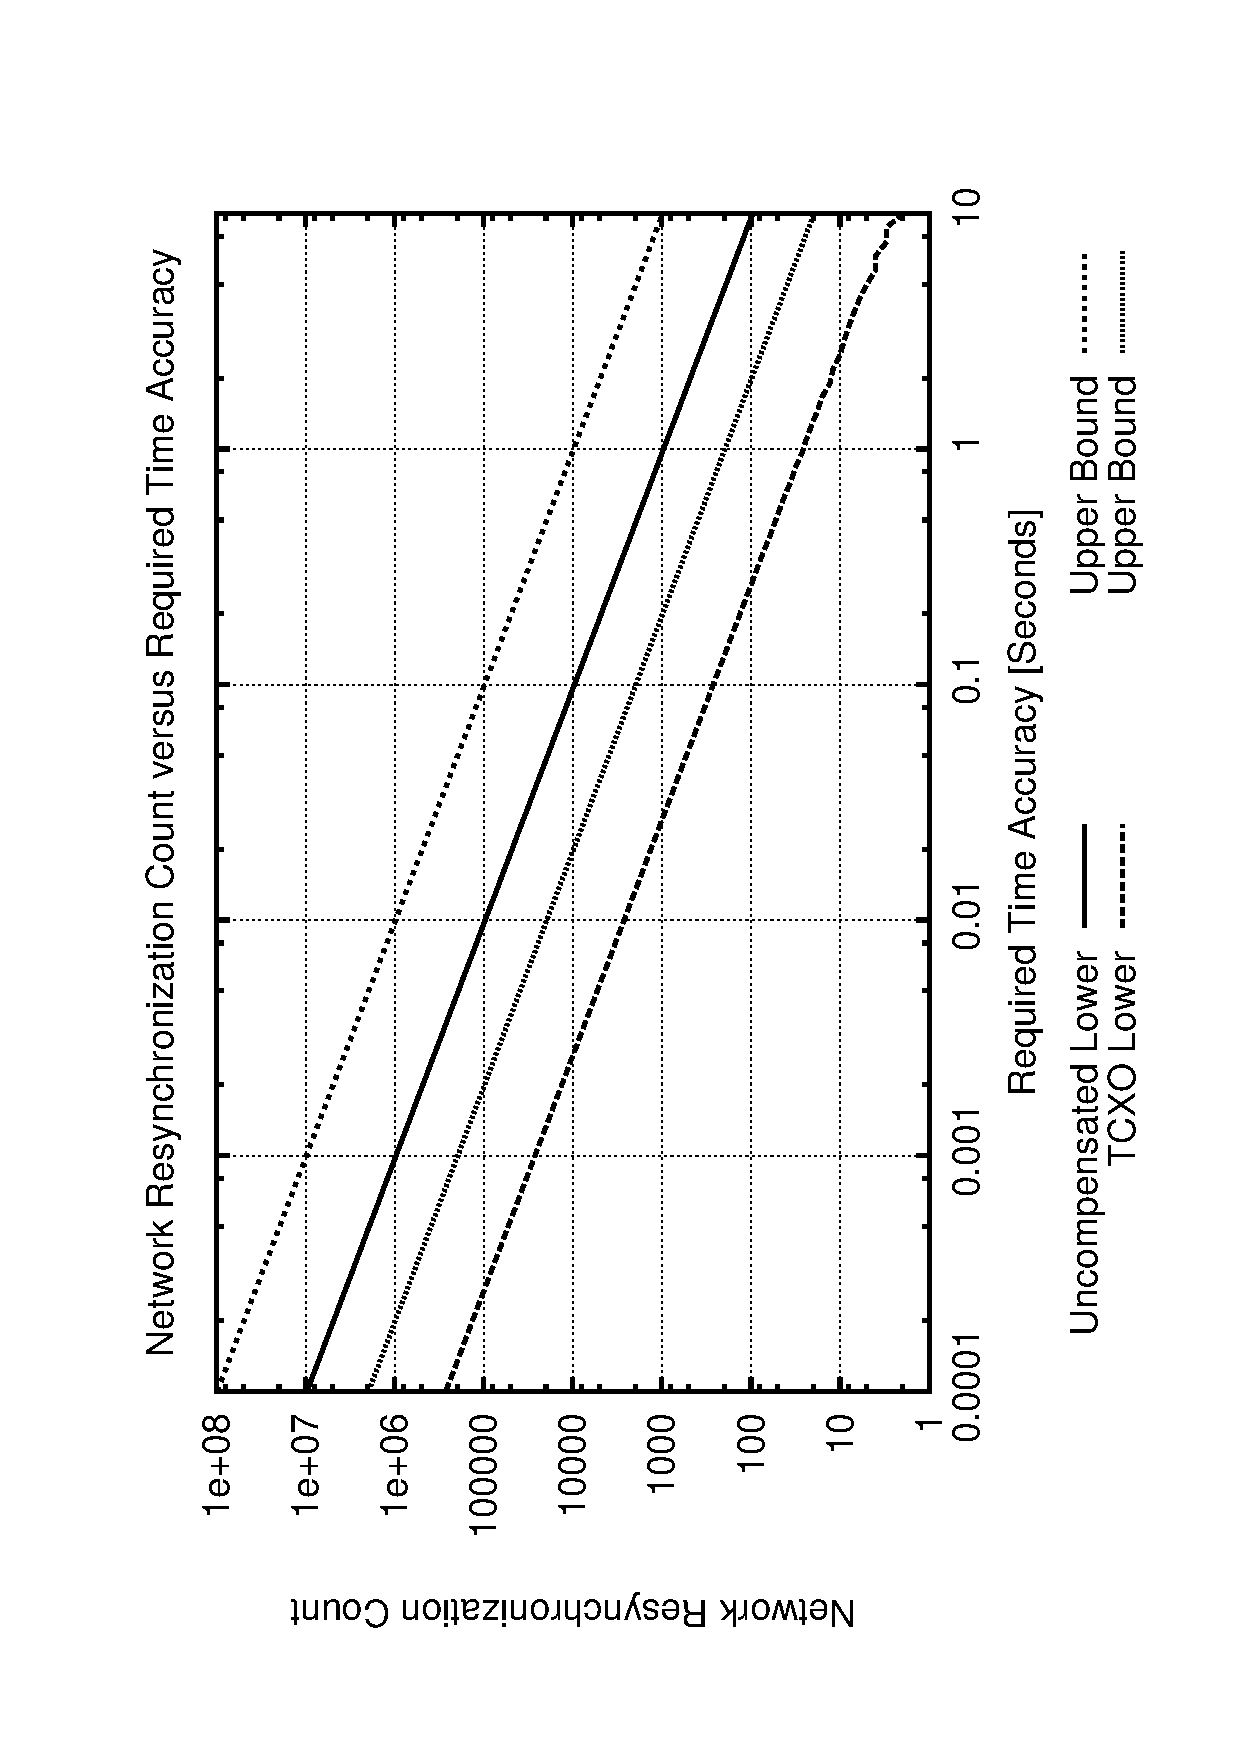
\includegraphics[angle=-90,width=0.45\textwidth]{figures/mosscamresync}
        \caption{Upper and lower bounds for the number of resynchronizations
        necessary to achieve a given time synchronization error. The
        temperature data comes from a 3 year dataset.}
        \label{fig:resync}
    \end{center}
\end{figure}

The question arises on what would be the optimal resynchronization interval
while still guaranteeing that the synchronization error is smaller than
$\epsilon$? Assuming the system has access to an oracle that tells the system
the current synchronization error, and that the system does not compensate for
local clock drift, it is clear that a system with a lower drift clock will
resynchronize less often than one with a higher drift. Figure \ref{fig:resync}
illustrates this by using a 3 year temperature dataset collected at the James
Natural Wildlife Reserve \cite{mosscam}. It shows the upper and lower bounds
by calculating how often a system would have to resynchronize experiencing the
temperature changes recorded in the dataset. Looking at one specific example,
we can calculate the bandwidth savings a better clock stability can achieve.
Let's assume that the application needs a synchronization accuracy of
$\epsilon<1ms$. Over the 3 year period, an uncompensated clock would have to
resynchronize at least 900'000 times using the oracle, whereas a compensated
TCXO only 25'000 times. Now, assuming that each resynchronization consists of
2 messages of 16 bytes each results in an average bandwidth of 2.35 bit/s for
the uncompensated clock, and only 0.065 bit/s for a compensated clock.

Even though this shows that a compensated clock can lower the number of
necessary resynchronizations, it does not mean that a time synchronization
system needs to employ a TCXO to achieve this compensation. Maroti et al.
showed in \cite{maroti2004ftsp} that FTSP can estimate the current clock drift
below an accuracy of 0.1ppm. Thus, as long as the environment temperature
doesn't change too often, drift compensation can be achieved in software to a
very high accuracy.

